\documentclass[11pt,a4paper]{article}

\setlength {\marginparwidth }{2cm}

\usepackage[margin=2.5cm]{geometry}
\usepackage{todonotes}
\usepackage[automake]{glossaries}
\usepackage{graphicx}
\usepackage{microtype}
\usepackage{listings}
\usepackage{color}
\usepackage{amssymb,amsmath}
\usepackage{mathpazo}
\usepackage{accents}
\usepackage{longtable,booktabs}
\usepackage{dcolumn}
\usepackage{pgf}
\usetikzlibrary{shapes.geometric}
\usetikzlibrary{matrix}
\usepackage{natbib}
\usepackage{hyperref}
\usepackage[capitalise,noabbrev,nameinlink]{cleveref}
\hypersetup{
  pdftitle={Proxy-key Solution Architecture},
  pdfborder={0 0 0},
  breaklinks=true
}

\definecolor{dkgreen}{rgb}{0,0.6,0}
\definecolor{gray}{rgb}{0.5,0.5,0.5}
\definecolor{pink}{rgb}{0.92,0.2,0.86}

\lstset{frame=tb,
  language=Haskell,
  aboveskip=3mm,
  belowskip=3mm,
  showstringspaces=false,
  columns=flexible,
  basicstyle={\ttfamily},
  numbers=none,
  numberstyle=\tiny\color{pink},
  keywordstyle=\color{pink},
  commentstyle=\color{pink},
  stringstyle=\color{pink},
  breaklines=true,
  breakatwhitespace=true,
  tabsize=3
}

\DeclareMathOperator{\dom}{dom}
\newcommand\restrict[2]{\left.#1\right||_{#2}}
\newcommand\deltavar[1]{\accentset{\Delta}{#1}}

\makeglossaries
\newglossaryentry{trustee}
{
    name={trustee},
    description={entity \emph{to whom} staking rights are being conferred}
}
\newglossaryentry{trustor}
{
    name={trustor},
    description={entity \emph{from whom} staking rights have been delegated}
}
\newglossaryentry{joint address}
{
    name={joint address},
    description={a Cardano address where both the payment and staking credentials used to forge the address are generated by \emph{both} the \gls{trustor} and \gls{trustee} respectively}
}

\begin{document}

\title {Proxy-key Solution Architecture Comparison \\
       {\large \sc An IOHK discussion paper}}
\date  {Version 0.2, 3rd February 2022}
\author{John Woods         \\ {\small \texttt{john.woods@iohk.io}} \\
                              {\small \texttt{john@postquantum.dev}} \\
}

\maketitle

\section{Purpose}
The purpose of this document is to present and contrast two viable approaches to the 
architectural design of \emph{Proxy-keys \& Partial delegation}. \\

The goal of the Proxy-keys feature is to protect cold key infrastructure, whilst
simultaneously providing a hot mechanism to manage stake delegation. As we will see herein, 
this hot mechanism should be capable of empowering not only the source Wallet owner, but also 
any 3rd party, to manage stake on behalf of the source Wallet owner. \\

This document will look at the requirements set forth by product, highlight the high-level
architecture of two possible solutions (the first Ledger based, the second Wallet based),
and finally, attempt to draw a conclusion as to which approach provides the most elegant,
scalable, robust and secure implementation.

\pagebreak

\tableofcontents

\pagebreak

\section{Acknowledgements}
The ideas presented herein are inspired by and based on discussions with
people from the research and engineering groups, specifically: Jared Corduan.

\section{Context}
Since the $Shelley$ release, a Cardano "Wallet" has two sets of keys. These keys
are both of type \lstinline{ed25519}, that is, the keys are used to create \lstinline{EdDSA}
signatures over the \lstinline{Edwards25519} elliptic curve.

\begin{enumerate}
  \item The first keypair is the payment key, which is used to control wallet funds.
  \item The second keypair is the staking key, which is used to manage stake delegation. 
\end{enumerate}

As of writing, with Daedalus, both keypairs are derived from the same $256-bit$ entropy
source, however this isn't a strict requirement. 
As outlined above, in current wallet implementations both payment and staking keys are tightly 
coupled. This means it's difficult (and at times impossible) to emancipate a staking key so 
that a 3rd party may control staking rights independently. 
To provide further context let's briefly review the Proxy-key feature requirements. \\

The ultimate goal is to develop a feature whereby staking rights may be transferred to a 3rd
party/entity, without losing control of the right to direct any generated rewards to an 
appropriate wallet, whilst concurrently obfuscating the source of staked funds. \\

Ergo, the required feature-set is approximately as follows:

\begin{itemize}
  \item Separate cold and hot infrastructure while managing stake delegation.
  \item Empower a \gls{trustee} with staking rights.
  \item Provide the source wallet privacy when delegating from Proxy-keys.
  \item Permit "partial delegation", so that a "single balance" of ADA may be delegated between multiple SPOs.
  \item Control the reward flow.
\end{itemize}

Whilst not discussed herein, the solution approach should attempt to consider "on-chain Voting",
despite the fact that a voting mechanism hasn't been fully designed nor implemented yet.
Voting/governance will be coming to Cardano, and it would be useful if voting rights could
also be proxied. Voting will (as staking does), likely employ a voting specific keypair.

\pagebreak

\section{Introduction}
Next we will consider two potential implementation approaches. The first of which will require modification 
to the Ledger layer of the core Cardano node. The second will require modification to the Wallet key 
management/generation logic. \emph{Both approaches will require modification to the Wallet UI}.

The overarching theme to both designs is one of simplicity. Whenever we are making changes we 
aim to provide a solution which is secure, robust and scalable, yet requires the lightest touch from an
implementation standpoint, to that end, both solutions have a focus on complexity reduction.

\section{Solutions}
Following is a high-level view of the technical architecture for both the Ledger and Wallet based solutions.
Ultimately our goal is to deliver on the functional and non-functional requirements, without adding
unnecessary complexity to the system components. Critically, we will also call out specific benefits \&
drawbacks, which should inform the approach choice.

\subsection{A Ledger based approach}
Conceptually, the Ledger based solution to deliver Proxy-keys is predicated on an extension of the existing
delegation mechanism. To begin, let us review how delegation is currently executed in the Ledger layer. 
Currently, users can formally stake their ADA balance to a given stake pool by posting a \emph{delegation certificate} 
to the blockchain.

\begin{description}
  \item A delegation certificate is a 2-tuple containing:
  \begin{itemize}
    \item the stake address delegating its stake rights, $\mathcal{A}_{s,\text{source}}$.
    \item the stake pool (verification key hash) to which stake is delegated, $\mathcal{H}(vk_\text{pool})$.
  \end{itemize}
  Posting a delegation certificate requires a signature from the private key counterpart of the delegating 
  stake address $\mathcal{S}(\mathcal{A}_{s,\text{source}})$.
\end{description} 

Next we propose an extension to this mechanism to satisfy the Proxy-key requirements.

\pagebreak

\subsubsection{High-level design}
Chiefly, the main enhancement to the existing delegation mechanism is the proposal of a \emph{Proxy delegation certificate}.

\begin{description}
  \item A Proxy delegation certificate is a 3-tuple containing:
  \begin{itemize}
    \item the stake address proxying its stake rights, $\mathcal{A}_{s,\text{source}}$, i.e. the \gls{trustor}.
    \item the stake address to which rights are being conferred, $\mathcal{A}_{p,\text{target}}$, i.e. the \gls{trustee}.
    \item the amount to be conferred upon the Proxy-key, $\mathcal{N}_{p,\text{index}}$.
  \end{itemize}
  Posting a proxy delegation certificate requires a signature from the private key counterpart of the source 
  stake address $\mathcal{S}(\mathcal{A}_{s,\text{source}})$.
\end{description} 

With this approach, we effectively create a "pointer" to the regular delegation certificate, which can be used to specify to the Ledger:
\begin{itemize}
  \item the identity of the \gls{trustee}.
  \item the amount the \gls{trustee} is empowered to stake.
  \item the identity of the \gls{trustor}.
  \item the approval of the \gls{trustor}.
\end{itemize}

This mechanism will allow us to meet most of the requirements described in the Proxy-key product requirements document,
however, it does have some limitations and indeed some complexities to be considered.

\subsubsection{Benefits \& drawbacks}
Next we will explore the benefits and drawbacks of the Ledger based solution described above. We will also explore
which requirements described in the PRD would be possible to meet.

\paragraph{Benefits:}
\begin{enumerate} 
  \item Capturing the complexity of the Proxy-key/partial delegation logic in the Ledger layer provides hooks to reduce the interactivity of the feature.
  \item Hardware wallets will not require additional development.
  \item We may be extending the role of on-chain certificates in the near term anyway.
\end{enumerate}

\paragraph{Drawbacks:}
\begin{enumerate} 
  \item With a Ledger based approach consider that once \emph{any} proxy delegation certificates are posted, the source stake key cannot be used to post a regular delegation certificate, as regular delegation certificates don't specify amounts. Thus, we would need a mechanism to "auto" proxy any partial balance to "self". This would result in either an implicit computational/accounting burden for Ledger or a monetary cost to the end-user to post apt proxy delegation certificates as their balance changes.
  \item This solution requires the full proxied balance to be delegated by the \gls{trustee}. 
  \item With a Ledger based approach consider that once \emph{any} proxy delegation certificates are posted, and the \gls{trustor} wishes to spend some amount $>n$, where $n$ is the balance which is \emph{not} proxied, we must take some undesirable action, such as:
  \begin{itemize}
    \item Immediately invalidate all proxied rights.
    \item Reissue all proxy delegation certificates with a new notional, reduced proportionally across all \glsplural{trustee}.
    \item Lock funds until manual action is taken. 
  \end{itemize} 
  \item Granular control over generated rewards is difficult to manage in a Ledger solution context, without further metadata being added to the proxy delegation certificates and a radical change to how the Ledger handles reward flows.
  \item A Ledger based solution will still require interactivity, i.e. sharing of the $\mathcal{A}_{p,\text{target}}$ public key/hash. To minimise interactivity we could define a request/response mechanism, however this would open a possible DDOS attack vector. 
  \item Privacy is difficult to achieve in a Ledger solution context. The chain is transparent by design and a Ledger based solution requires posting data to the chain. Privacy would require implementation of a zero knowledge proving/verification system between all parties using the chain.
  \item A Ledger based solution does not avoid changes to the Wallet. 
\end{enumerate}

\pagebreak

\subsection{A Wallet based approach}
Conceptually, the Wallet based solution to deliver Proxy-keys is predicated on the notion of creating a 
\gls{joint address} comprised of both a \gls{trustor} and \gls{trustee} component. Let us remind ourselves how 
a Cardano \emph{Shelley}-era address is generated:

\begin{figure}[ht]
  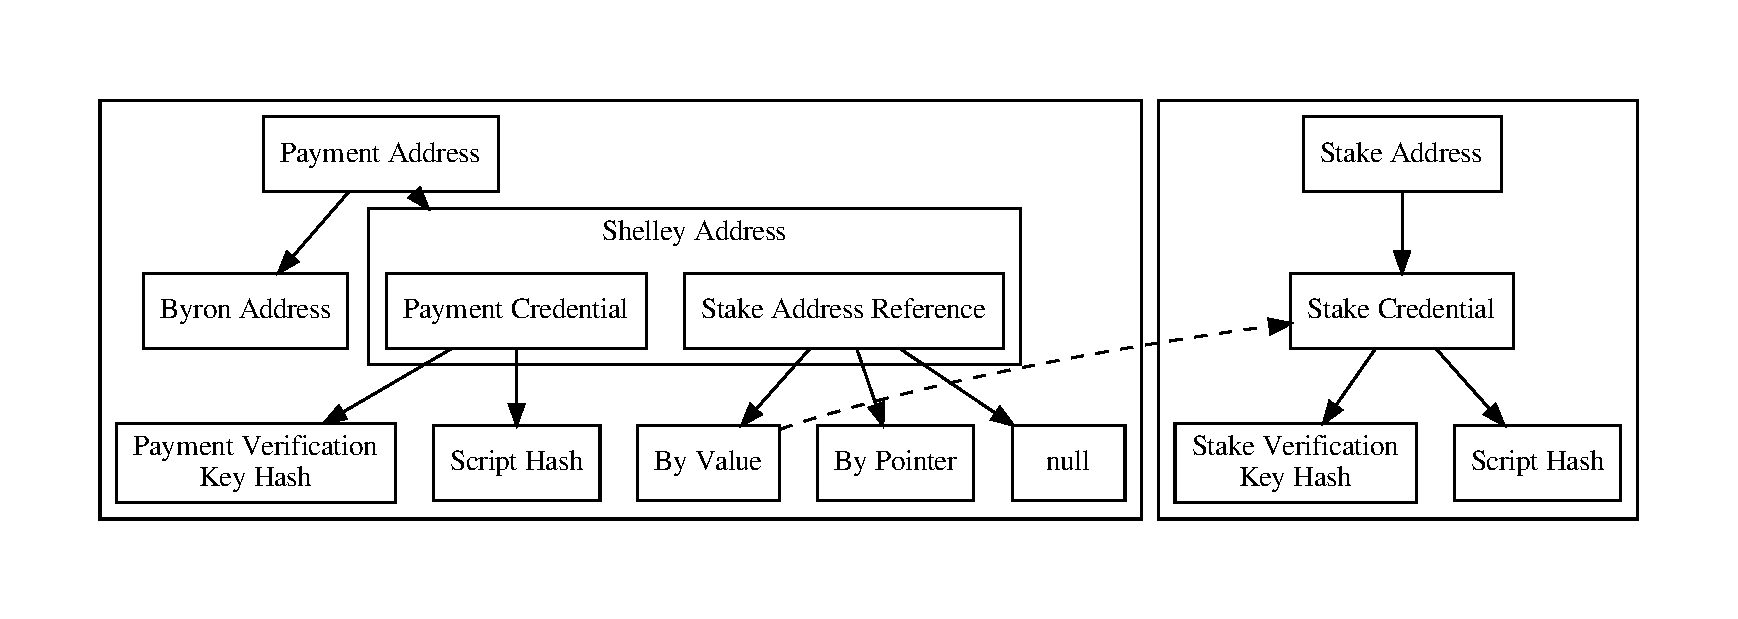
\includegraphics[width=\linewidth]{images/addresses.pdf}
  \caption{address/credential interaction - from SL-D1}
  \label{fig:addresses}
\end{figure}

As shown above the structure of a Shelley-era address (from which one can delegate stake), is forged from a 
\emph{payment credential}, $\mathcal{A}_p$ and a \emph{stake credential}, $\mathcal{A}_s$. With the current 
core Cardano protocol, the payment credential, (or more accurately the credential's private key counterpart), 
controls the spending of funds, and the stake credential controls delegation/de-delegation and withdrawal of 
rewards from the account they accumulates to. \\

\subsubsection{High-level design}
Cognisant of the above, the solution to deliver the Proxy-key/partial delegation feature is to deposit funds
to an address which is formed from two distinct, separately created keypairs both of type \lstinline{ed25519}.
The \gls{trustor} public credential forms the "payment" side of the \gls{joint address}, and the 
\gls{trustee} public credential forms the "stake" side of the \gls{joint address}. This will ultimately yield
a wallet where the \gls{trustor} has sole control of spending rights, whilst the \gls{trustee} enjoys sole
staking rights. The mechanism of delegating to a given stake pool will remain unmodified, by posting a \emph{delegation 
certificate} to the blockchain. \\

We can use hardened key derivation, by performing a \lstinline{BLAKE2b} hash on the \gls{trustor} \& \gls{trustee}
private keys: $\mathcal{H}(\mathcal{A}_{(x)})$, where $_{(x)}=\mathcal{A}_p$, or $\mathcal{A}_s$. 
This will yield the ability to create an arbitrary number of proxy wallets from $2$ independently
stored seeds, which makes wallet recovery trivial. \\

Finally, if we use the hash of a \emph{Plutus script} as the \emph{stake credential} component during the process outlined
above, then we can enjoy granular control over any \emph{rewards} generated. Including both permitting or restricting
withdrawal of rewards by the Proxy-key. Plutus scripts have context. They understand whether an action is Spending, 
Minting, Delegating or Rewarding, thus, we can express conditional logic which finely controls actions executed by the \gls{trustee} Proxy-key.

\pagebreak

\subsubsection{Benefits \& drawbacks}
Next, again, we will explore the benefits and drawbacks. This time of a Wallet based solution. We will also explore
which requirements described in the PRD would be possible to meet.

\paragraph{Benefits:}
\begin{enumerate} 
  \item Leverages existing Ledger primitives (Shelley design), so we don't require a protocol hard-fork, nor do we add complexity to the core node.
  \item Controlling reward flow is trivial using Plutus scripts.
  \item There is no further computational/accounting burden on the core Cardano node. 
  \item There is no complex management needed when a \gls{trustor} spends funds in the context of proxy to multiple \glsplural{trustee}.
  \item There is no need to proxy delegate a partial balance back to self.
  \item This approach will likely dovetail well with the expected voting implementation.
  \item All requirements of the Proxy-key PRD can be met, including privacy, with reasonable implementation effort.
\end{enumerate}

\paragraph{Drawbacks:}
\begin{enumerate} 
  \item Hardware wallets will require development to support Proxy-keys.
  \item Additional development would be required by all software wallets to support the Proxy-key feature.
  \item There is no hook to provide a non-interactive UX.
\end{enumerate}

\pagebreak

\section{Considerations \& conclusion}
Both solutions designs are viable approaches to implement the Proxy-keys feature. Additionally, both designs have
individual benefits and drawbacks. Notwithstanding, there are some specific considerations which should influence our decision
as to which approach is selected:

\begin{itemize}
  \item Ultimately, both the Ledger based approach and the Wallet based approach require interactivity in some form, though this could be hidden from the user in the case of a Ledger based solution.
  \item Both approaches will require knowledge of the trustee's Proxy-key public curve point which would then either be:
    \begin{itemize}
      \item formed into a stake credential and subsequently combined with the appropriate payment credential to form a \gls{joint address}, or;
      \item embedded into a proxy delegation certificate and posted to the chain.
    \end{itemize}
    \item Privacy is an important aspect to the solution, Ledger based privacy is going to significantly increase delivery time for the feature. 
    \item Control of reward flow is an important aspect to the solution, which is significantly easier to achieve in a Wallet based solution, via Plutus.
    \item Both solution approaches will require development work in the Wallet. 
    \item A Wallet based approach simplifies accounting in the context of proxy to multiple \glsplural{trustee}.
  \end{itemize} 

\textbf{ \\ \\ Mindful of the discussion points herein, the recommendation from Architecture and Engineering is to pursue a Wallet
based solution to implement Proxy-keys \& Partial delegation}.
\pagebreak

\printglossaries

\end{document}